\begin{pro}
  Consider a finite difference solution of the Poisson equation
  $u_{xx}+u_{yy}=x+y$ on the unit square using the boundary
  conditions and mesh points shown in the drawing.
  Use a second-order accurate,
  centered finite difference scheme to compute the approximate
  value of the solution at the center of the square.
  \begin{figure}[H]
    \centering
    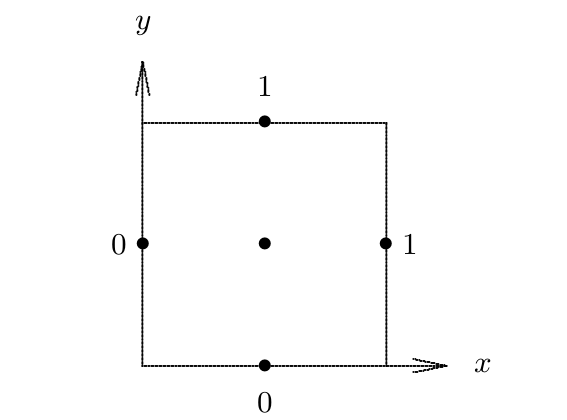
\includegraphics[scale=0.25]{poisson.png}
  \end{figure}
\end{pro}

\begin{sol}
  \begin{align*}
    & \frac{u_{2,1}-2u_{1,1}+u_{0,1}}{h_x^2} +
      \frac{u_{1,2}-2u_{1,1}+u_{1,0}}{h_y^2} = x_1 + y_1 \\
    \Rightarrow & u_{1,1} = \frac{u_{2,1}+u_{0,1}+u_{1,2}+u_{1,0}-h^2(x_1+y_1)}{4} \\
    \Rightarrow & u_{1,1} = \frac{7}{16}.
  \end{align*}
\end{sol}
%%% Local Variables:
%%% mode: latex
%%% TeX-master: "../hw5"
%%% End:
